\begin{minipage}{0.95\columnwidth}
\begin{figure}[tb]
\centering
\begin{subfigure}[t]{0.47\textwidth}
    \centering
    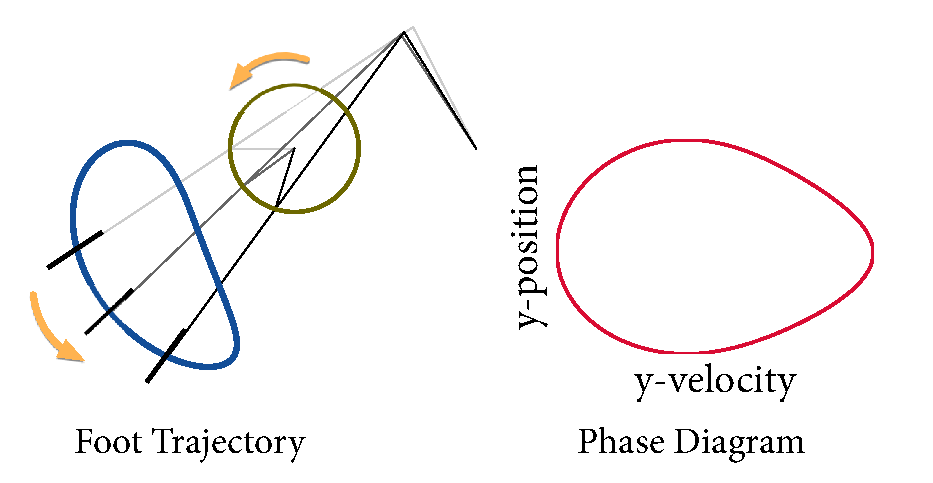
\includegraphics[width = \textwidth]{foot_traj_orig.eps}
    \caption{Real Foot locus and phase portrait. The circular path traced by end of the input link is traced in green.} 
    \label{fig:trajrob}
\end{subfigure}
\quad
\begin{subfigure}[t]{0.47\textwidth}
    \centering
    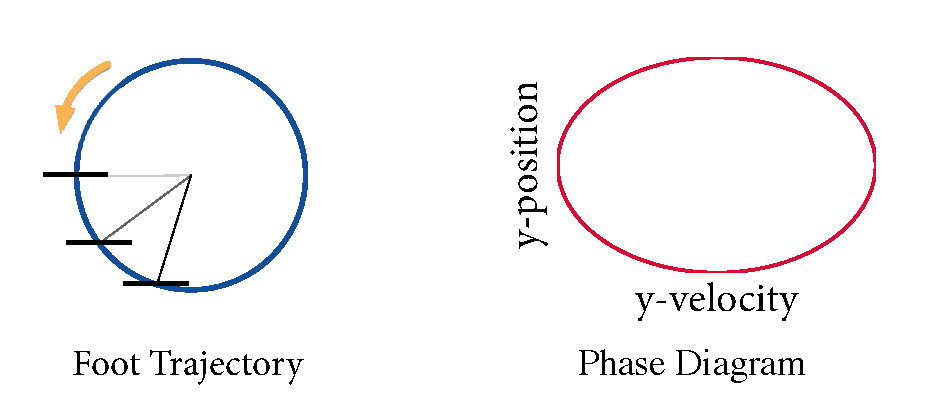
\includegraphics[width = \textwidth]{foot_traj_simple.eps}
    \caption{Simplified foot locus and phase portrait.} 
    \label{fig:trajsimp}
\end{subfigure}
\caption{Real and simplified leg trajectories (blue) and phase portraits (red).}
\label{fig:traj}
\end{figure}
\end{minipage}
\vspace{1EX}

\textcolor{prime}{\textsf{Leg Model}}
\begin{itemize}
    \item Only considers vertical forces
    \item Uses the average force generated in one leg cycle
    \item Assumes velocity of leg $>>$ velocity of body oscillations
    \item Allows for different foot velocties during downwards and upwards phases of trajectory
    \item We integrate the following force equation~\cite{glasheen1996vertical}
        \begin{equation}
            F(t) = - C_D^* \left[\frac{1}{2} S \rho \dot{y}_f(t) |\dot{y}_f(t) | + S \rho g y_f(t) \right]
            \label{eq:force_t}
        \end{equation}
\end{itemize}

\textcolor{prime}{\textsf{Robot Model}} \\
We linearize the result of integrating equation~\ref{eq:force_t} over the trajectory and write the height and roll dynamics in the form

\begin{equation}
    M \ddot{\vec{y}} = A \vec{y} + G + B \vec{\omega} 
    \label{eq:rob_dyn}
\end{equation}

$\vec{y} = [y, \theta]^T =  [\textrm{height}, \textrm{roll}]$\\
$\vec{\omega} = $ upwards and downwards leg frequencies for left and right sides of robot
